% Descripción de estos servidores 
Un servidor de archivos permite a los usuarios compartir información a través de una red sin tener que transferir físicamente los archivos por algún medio de almacenamiento externo extraible.
\subsubsection{Instalación del servidor}
Utilizamos en esta parte el servidor VSFTPD para hacer la transferencia de archivos mediante el protocolo FTP. Los pasos para su instalación son los siguientes:
\begin{figure}[!htbp]
	\hypertarget{fig:instalacionFTP}{\hspace{1pt}}
	\begin{center}
		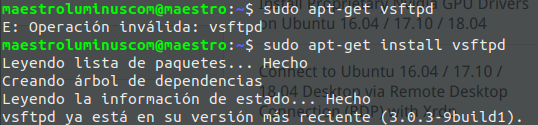
\includegraphics[width=0.7\textwidth]{desarrollo/tarea2/img/instalacionFTP.png}
		\caption{Instalamos el servidor VSFTPD.}
		\label{fig:instalacionFTP}
	\end{center}
\end{figure}
\pagebreak
\begin{figure}[!htbp]
	\hypertarget{fig:modificarFTP}{\hspace{1pt}}
	\begin{center}
		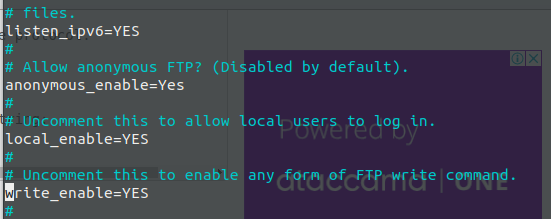
\includegraphics[width=0.7\textwidth]{desarrollo/tarea2/img/modificarFTP.png}
		\caption{Modificamos el archivo de configuración vsftpd.conf.}
		\label{fig:modificarFTP}
	\end{center}
\end{figure}
\pagebreak
\begin{figure}[!htbp]
	\hypertarget{fig:servicioFTP}{\hspace{1pt}}
	\begin{center}
		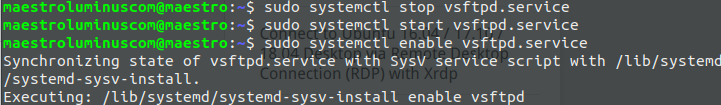
\includegraphics[width=0.7\textwidth]{desarrollo/tarea2/img/servicioFTP.png}
		\caption{Habilitamos el servicio VSFTPD.}
		\label{fig:servicioFTP}
	\end{center}
\end{figure}
\subsubsection{Sensor}
Este sensor se escribió en Bash. Toma como parámetros de entrada el servidor al que se le va a hacer la petición, el usuario de FTP, su contraseña y el nombre del archivo que se desea ardquirir.
\begin{figure}[!htbp]
	\hypertarget{fig:sensorFTP}{\hspace{1pt}}
	\begin{center}
		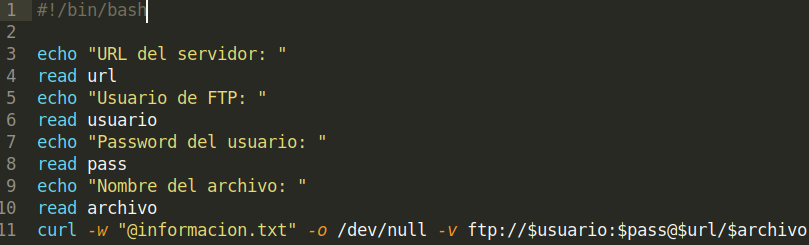
\includegraphics[width=0.7\textwidth]{desarrollo/tarea2/img/sensorFTP.png}
		\caption{Código del sensor FTP.}
		\label{fig:sensorFTP}
	\end{center}
\end{figure}

Después de ejecutarse el archivo, la salida es la siguiente.

\pagebreak
\begin{figure}[!htbp]
	\hypertarget{fig:outputFTP}{\hspace{1pt}}
	\begin{center}
		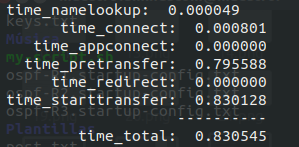
\includegraphics[width=0.7\textwidth]{desarrollo/tarea2/img/outputFTP.png}
		\caption{Salida de la ejecución del sensor FTP.}
		\label{fig:outputFTP}
	\end{center}
\end{figure}